\patchcmd{\appendices}{\quad}{: }{}{}
\begin{appendices}

\section{Research Paper Lucas Gehlen: Object-Oriented Programming vs Functional Programming}
\label{appendix:research_paper_lucas_gehlen}

The following pages contain the research paper \textit{"Object-Oriented Programming vs Functional Programming"}, written by the co-author Lucas Gehlen. It details what the differences between Object-Oriented Programming and Functional Programming are and when to use which paradigm. 

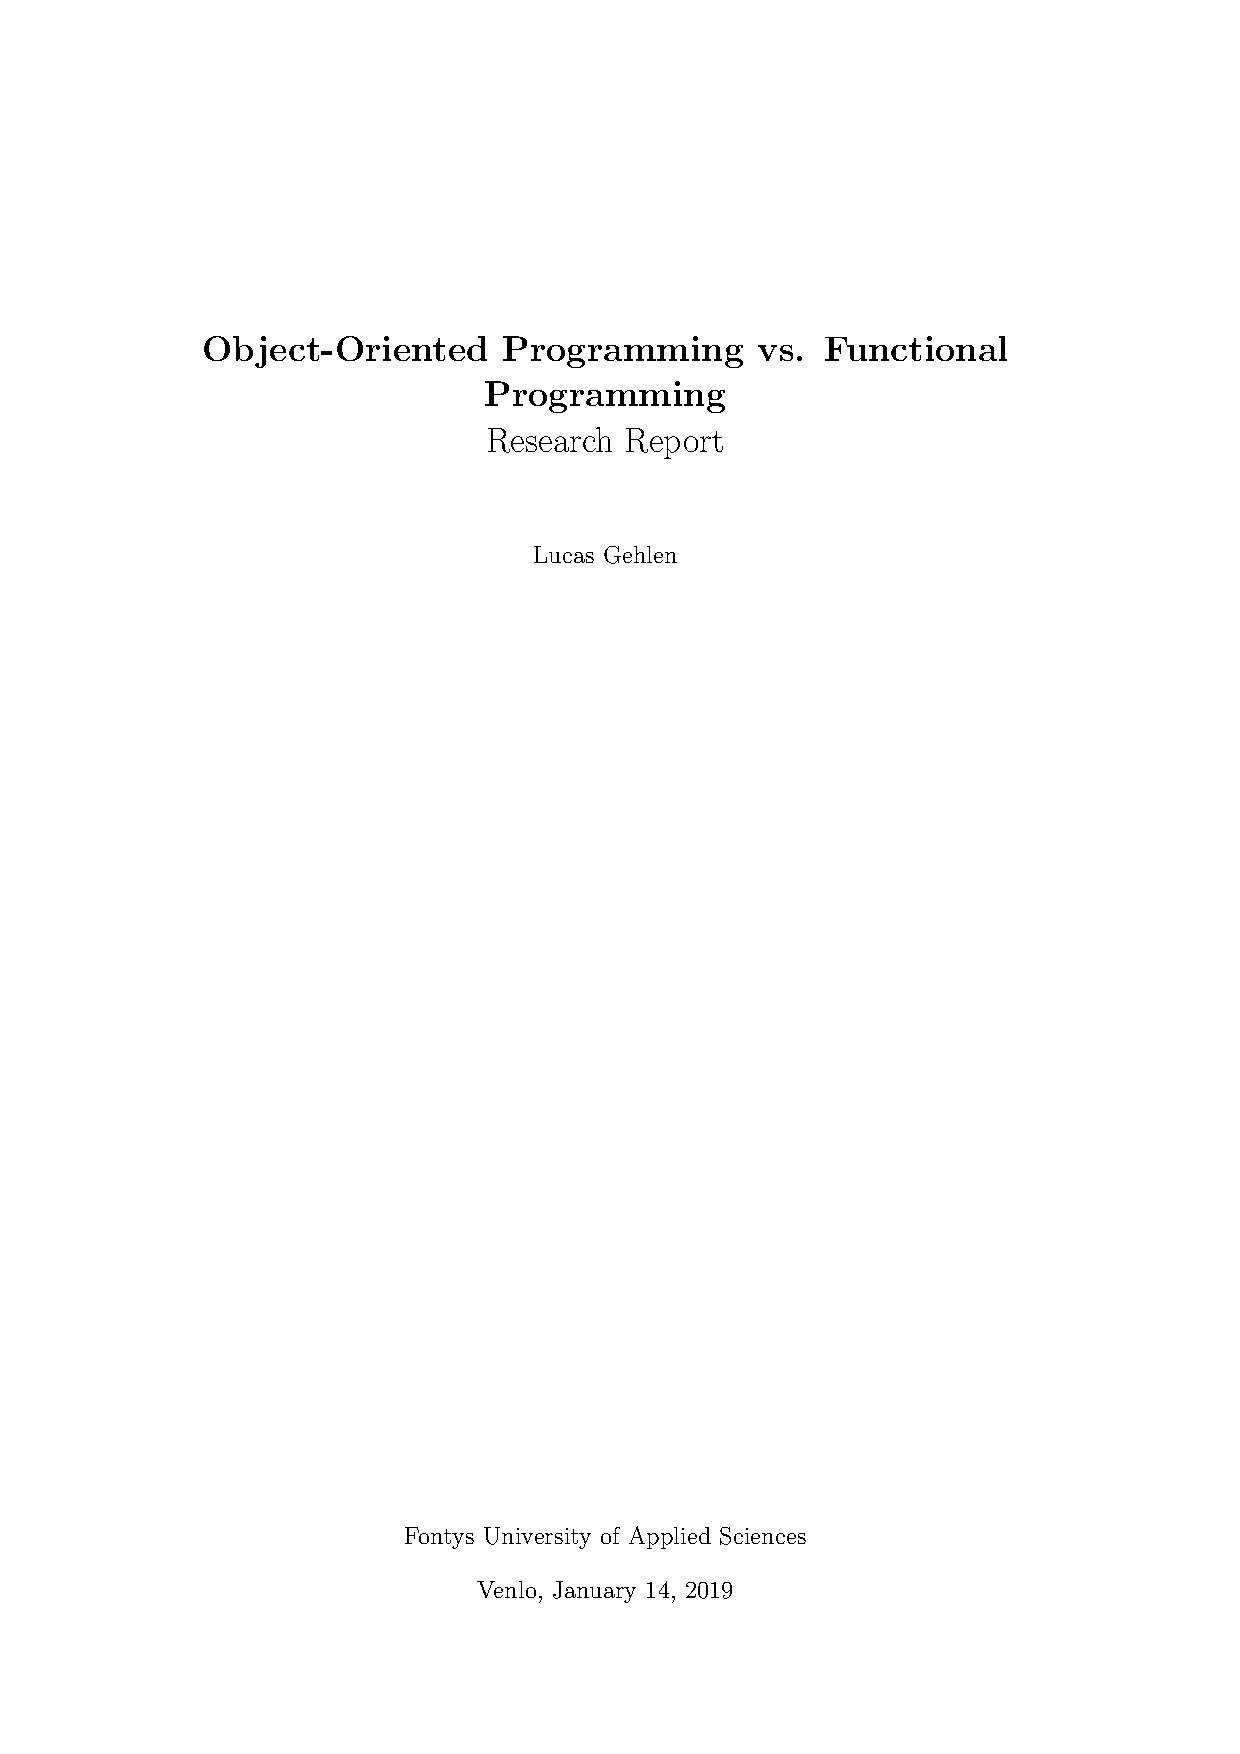
\includepdf[pages=-]{additional/research_oop_vs_fp} 

\newpage

\section{Research Paper Marco Kull: SQL vs. NoSQL}
\label{appendix:research_paper_marco_kull}

The following pages contain the research paper \textit{"SQL vs. NoSQL"}, written by the co-author Marco Kull. It details different designs of NoSQL databases and a comparison between \textit{SQL} and \textit{NoSQL} databases.

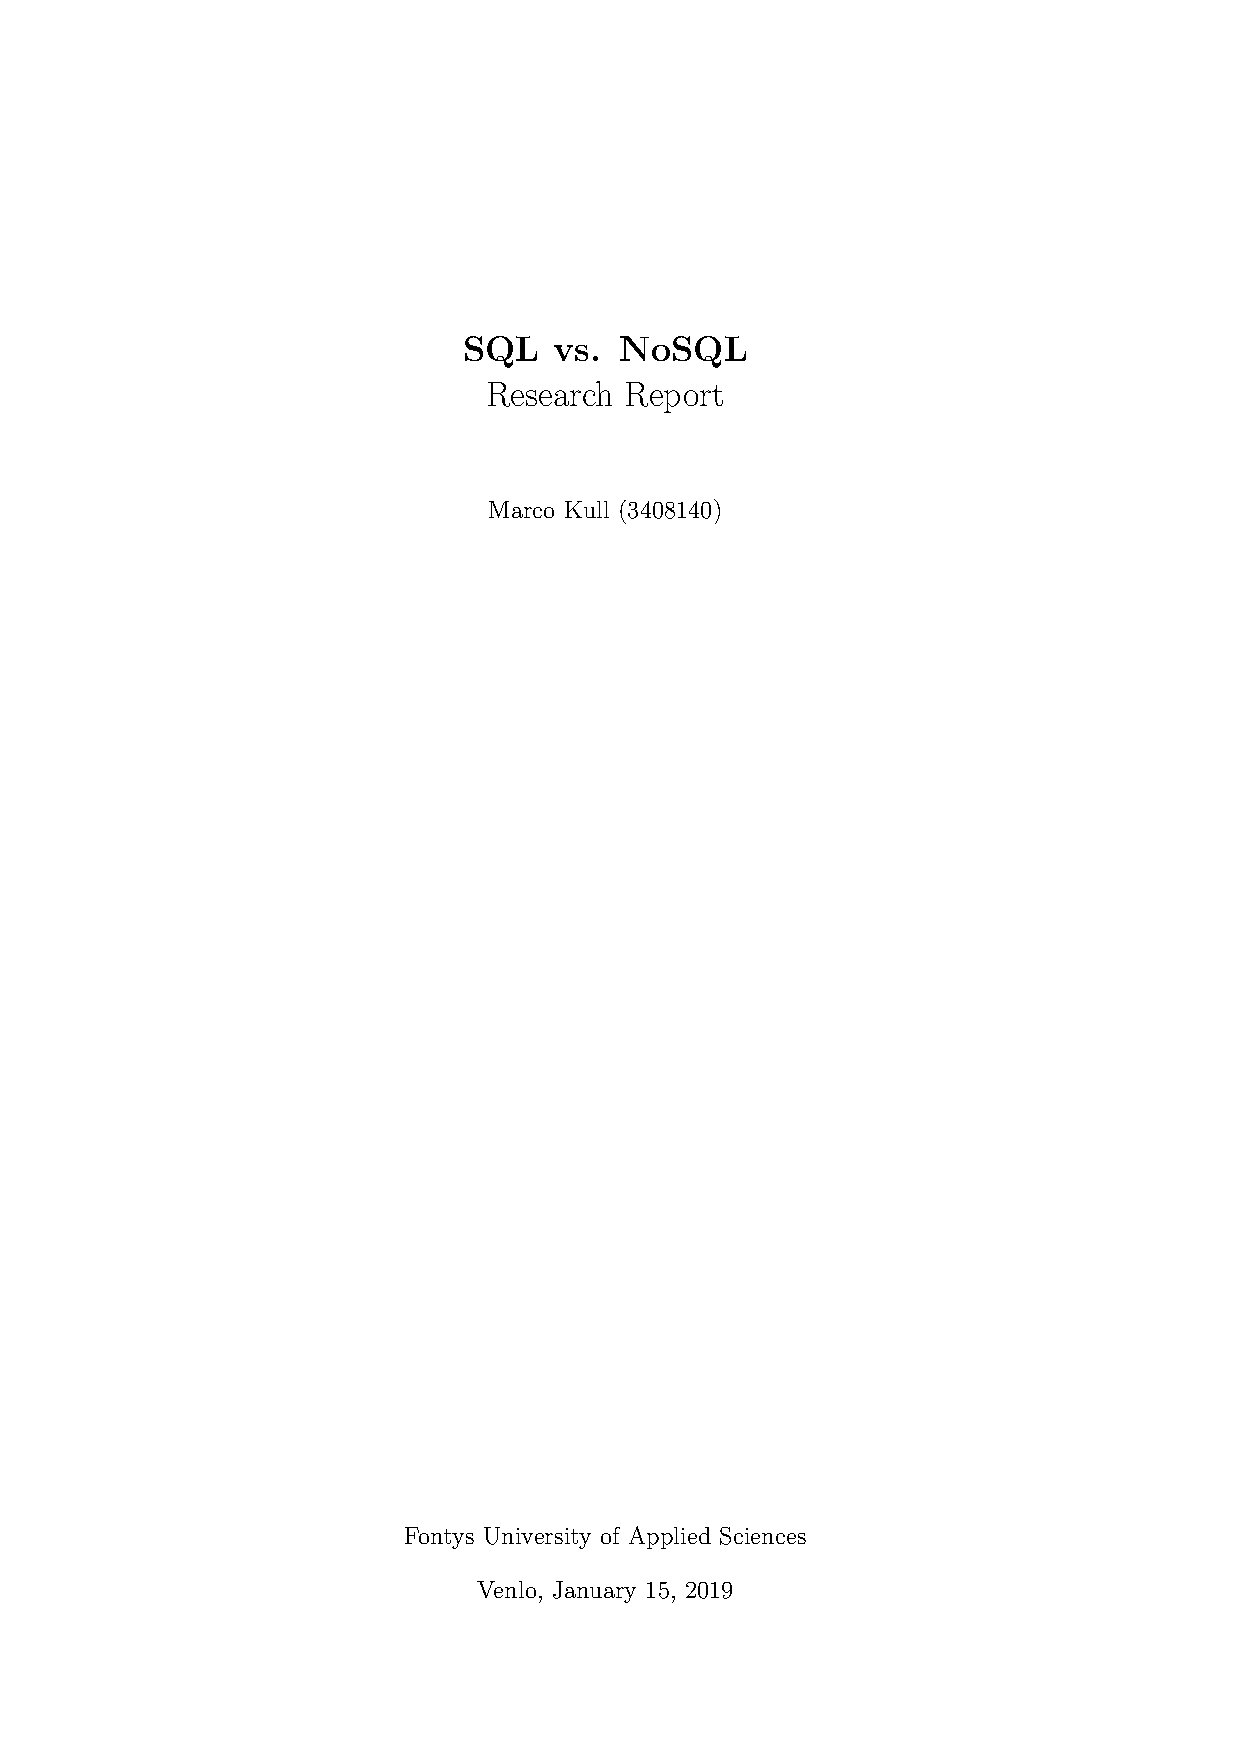
\includepdf[pages=-]{additional/research_sql_vs_nosql} 

\newpage

\section{Research Paper Patrick Richter: GraphQL}
\label{appendix:research_paper_patrick_richter}

The following pages contain the research paper \textit{"GraphQL"}, written by the co-author Patrick Richter. It details the advantages and disadvantages of \textit{GraphQL} as well as it's usage.


\includepdf[pages=-]{additional/research_report_patrick_richter_graphql} 

\newpage

\section{Research Paper Sebastian Wilczek: End-To-End Testing for React Native Applications}
\label{appendix:research_paper_sebastian_wilczek}

The following pages contain the research paper \textit{"End-To-End Testing for React Native Applications"}, written by the co-author Sebastian Wilczek. It details different frameworks that can be used to end-to-end test \textit{React Native} applications, both in general context as well as in the context of the \textit{Connected.Football} application.

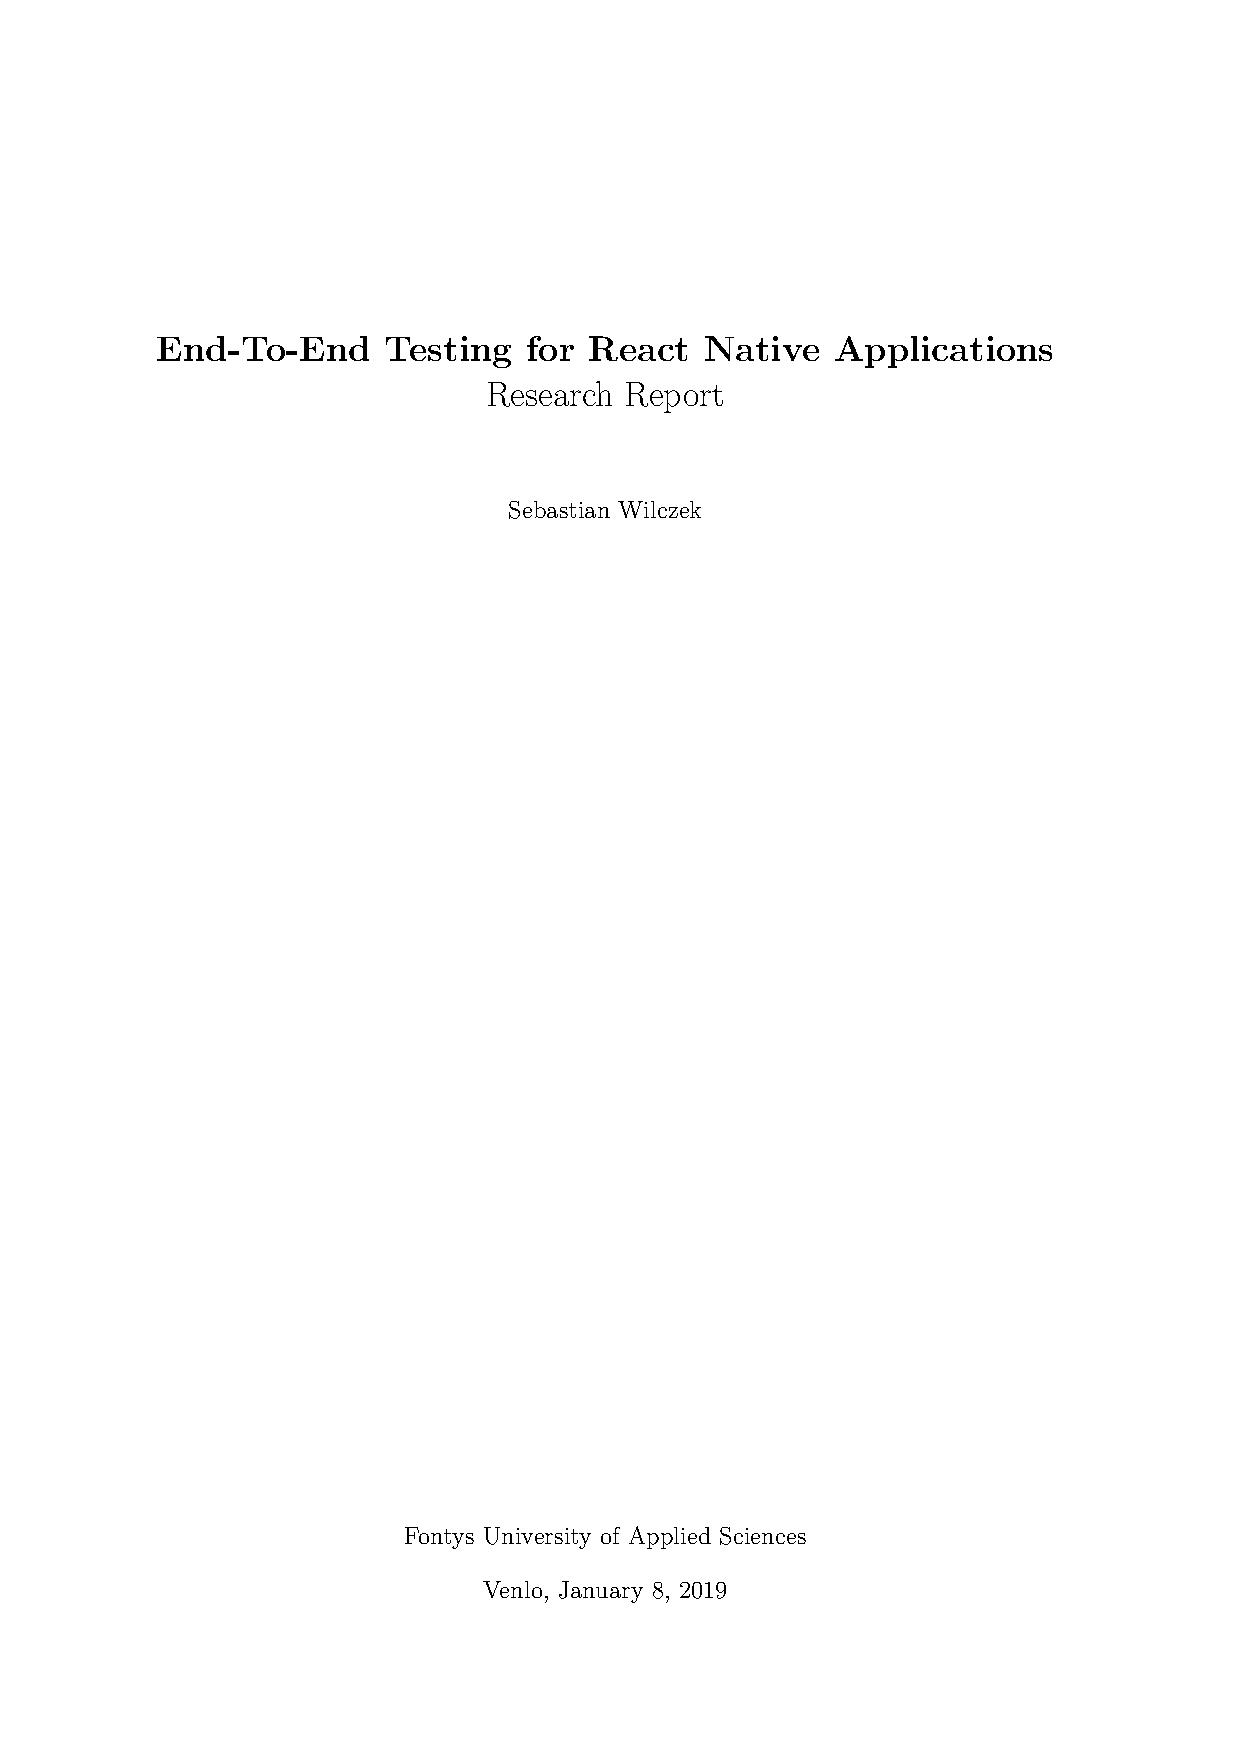
\includepdf[pages=-]{additional/research_report_sebastian_wilczek_end_to_end_testing_for_react_native_applications}

\newpage

\section{Handover Document}
\label{appendix:handover_document}

The following pages contain the handover document of the \textit{Connected.Football} project, written by all co-authors. It is intended to be read as a "quick start" to resume work on the \textit{Vote4Fun} development.

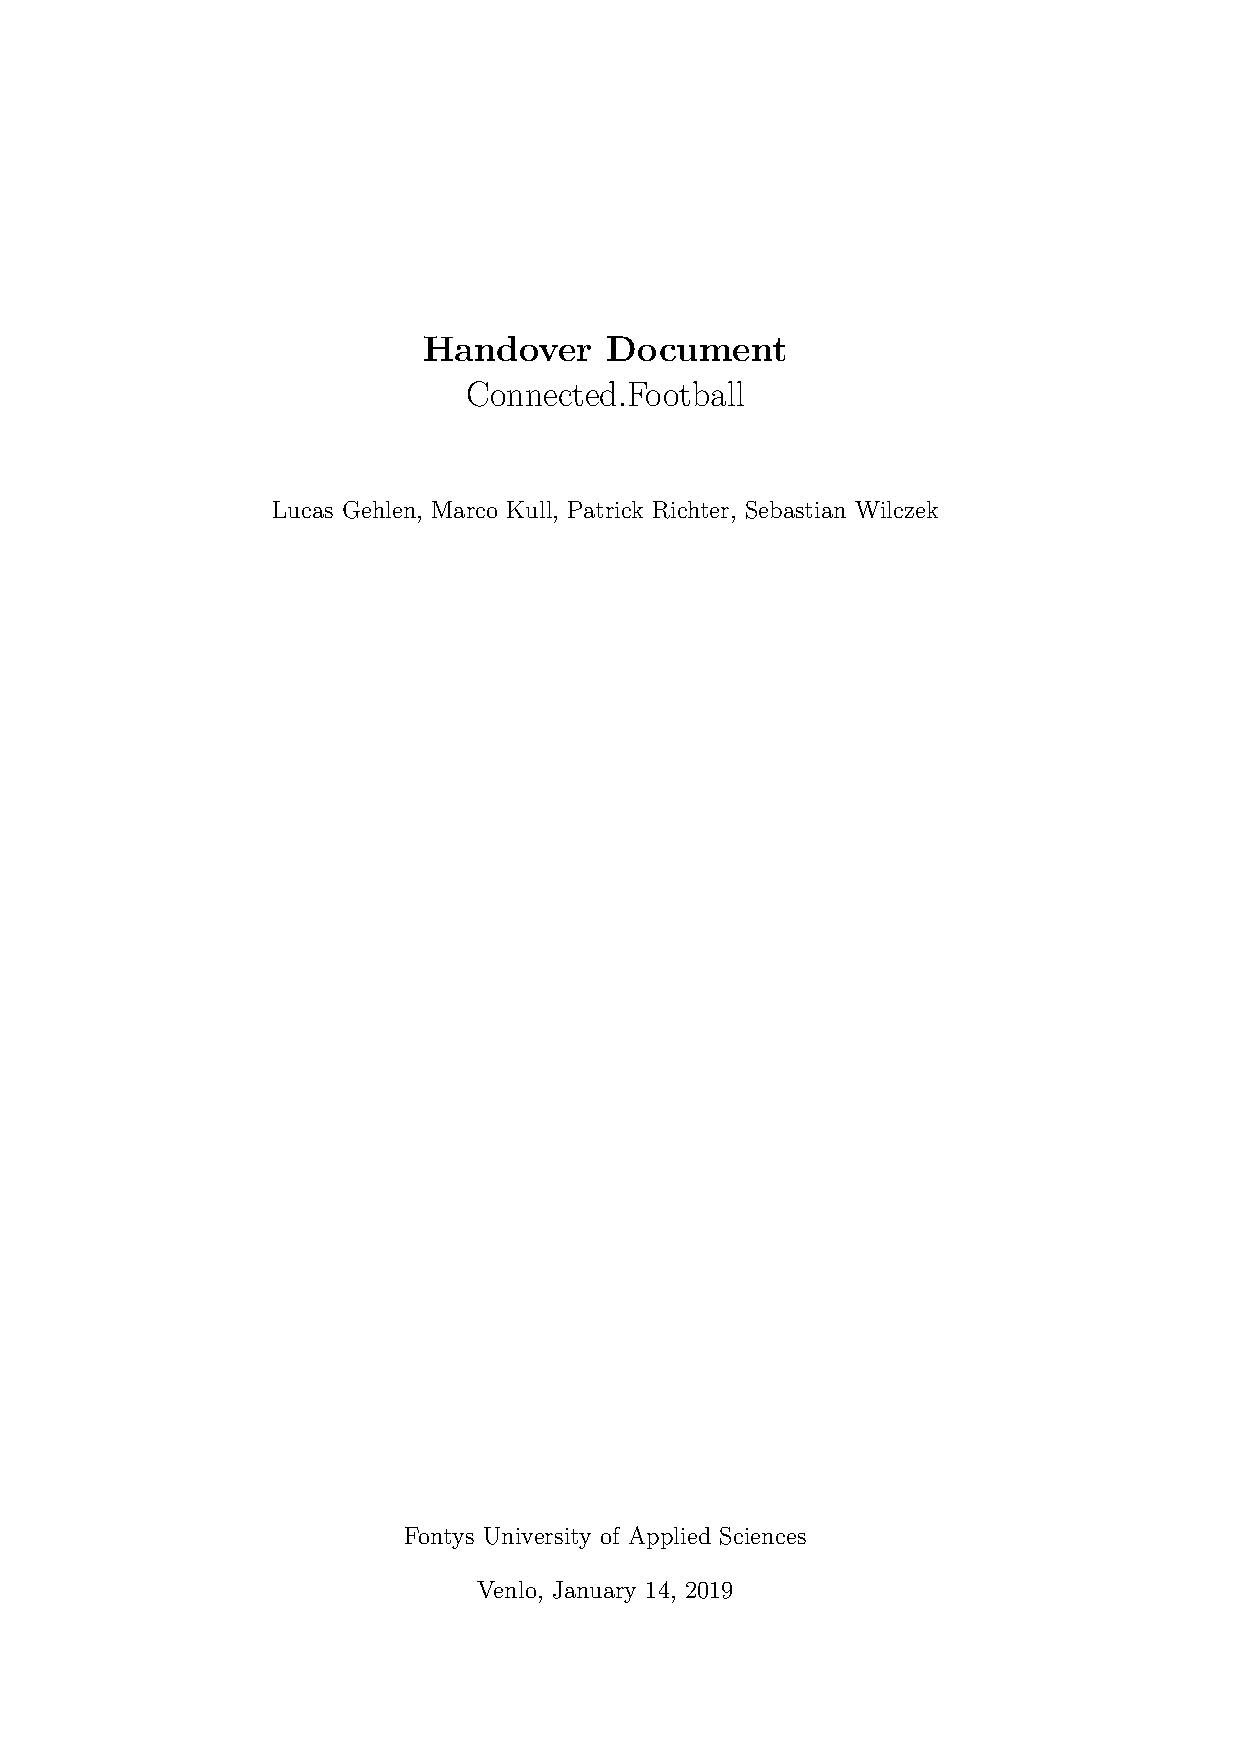
\includepdf[pages=-]{additional/Handover_Document_Connected_Football}

\newpage

\section{Project Pitch Video}
\label{appendix:pitch_video}

A pitch video that present the idea behind the project and the functionality of the implemented product was created as a deliverable. This video is intended to be watched by interested parties to introduce them to the \textit{Vote4Fun} extension and to peak interest.
\newline
The video itself was uploaded to YouTube. It can be found under the following link: \url{https://www.youtube.com/watch?v=lAWgD2TyeZE}

\newpage

\section{Software Requirements Specification}
\label{appendix:srs}

The following pages contain the Software Requirements Specification that was made to describe the requirements for the first epic.

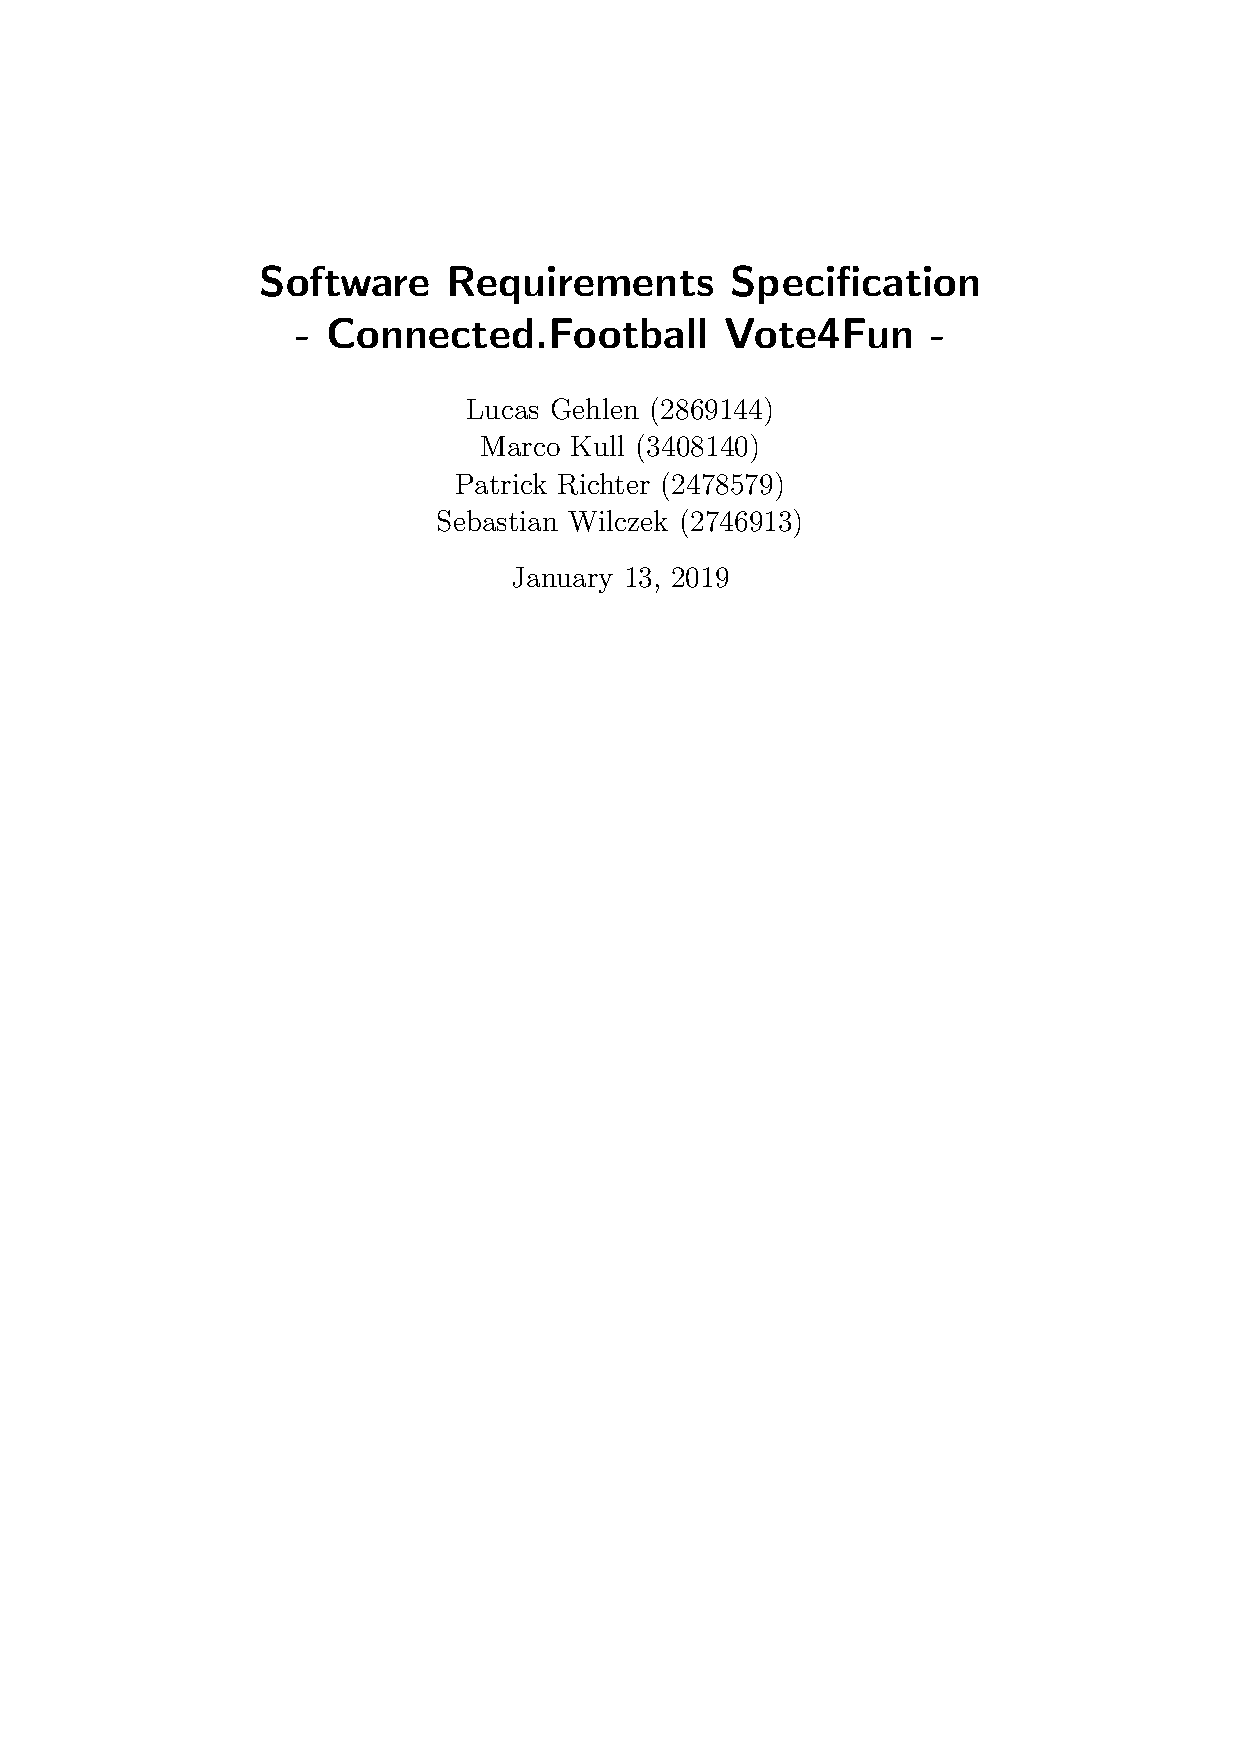
\includepdf[pages=-]{additional/srs}

\end{appendices}